\chapter{Applicazione}

In questo capitolo saranno esposti i requisiti dell'applicazione, seguiti da una breve analisi e progettazione di un sistema che li implementa.

\section{Requisiti}
L'obiettivo principale è quello di poter definire e analizzare modelli virtuali di incrocio stradale, in modo da riuscire ad effettuare aggiustamenti sul traffico e quindi minimizzare l'impatto che può avere un mezzo come la tramvia sulla circolazione degli altri veicoli.

Per mantenere generale l'applicazione, dovrà essere possibile la descrizione di porzioni più ampie di mappa stradale in modo da supportare analisi di tipo diverso, nonché eventuali simulazioni.

In questo lavoro saranno realizzate le seguenti analisi esemplificative:
\begin{itemize}
	\item Disponibilità di un incrocio: la probabilità che le auto siano libere di procedere, ovvero che il semaforo sia verde.
	\item Lunghezza media di una coda: Considerando alcuni fattori come il tempo di attraversamento, si vuol sapere quale sarà la dimensione della coda delle auto.
	\item Tasso di overflow: Caso in cui un'auto non riesce ad entrare nella via a causa del traffico eccessivo.
\end{itemize}

Tramite il software sarà possibile definire, oltre alla topologia della rete stradale, una serie di parametri necessari all'analisi di essa.
Alcuni dei valori gestiti saranno:
\begin{itemize}
	\item Periodo dell'analisi: cadenza con la quale i treni arrivano in prossimità dell'incrocio;
	\item Eventuale ritardo di arrivo del tram;
	\item Tasso di arrivo delle auto;
	\item Tempo di attraversamento delle auto;
	\item Dimensione massima della coda (calcolabile dalla lunghezza del tratto di strada e dalla dimensione dei veicoli);
	\item Tempo di attraversamento del tram;
	\item Tempo di anticipo del semaforo rispetto all'arrivo; effettivo del treno;
\end{itemize}

Sempre con lo scopo di supportare analisi non ancora stabilite, sarà possibile impostare sui vari elementi della rete un numero arbitrario di parametri.
Questi saranno suggeriti dagli stessi moduli di analisi.


\section{Casi d'uso}

Sono state individuate tre categorie di utilizzatori (vedi figura \ref{fig:uc-users}):
\begin{itemize}
	\item Amministratore
	\item Esperto
	\item Cliente
\end{itemize}

\begin{figure}[h]
	\centering
	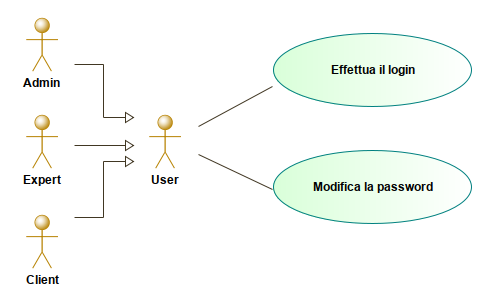
\includegraphics[scale=0.5]{img/UserUC}
	\caption{Classificazione degli utenti}
	\label{fig:uc-users}
\end{figure}

Ogni utente potrà accedere all'applicazione tramite una funzionalità di login, così da avere accesso alle aree del software di propria competenza, nonchè alla sezione di gestione del profilo.

Gli utenti di tipo \textit{amministratore} hanno la possibilità di gestire gli accounts aggiungendone di nuovi o eliminandone di esistenti (figura \ref{fig:uc-admins}).
Per semplicità sarà lo stesso amministratore a stabilire le password iniziali, che potranno essere modificate in seguito dai proprietari.

\begin{figure}[h]
	\centering
	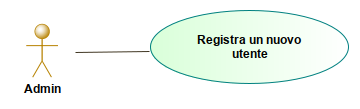
\includegraphics[scale=0.5]{img/AdminUC}
	\caption{Casi d'uso di un amministratore}
	\label{fig:uc-admins}
\end{figure}

Gli utenti \textit{esperti} conoscono a fondo il dominio e sono in grado di configurare un modello specificando le varie proprietà.
Per questo hanno il permesso di definire valori di default o complete configurazioni per gli utenti meno esperti (figura \ref{fig:uc-experts}).

\begin{figure}[h]
	\centering
	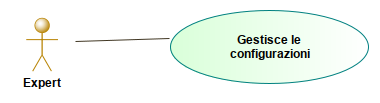
\includegraphics[scale=0.5]{img/ExpertUC}
	\caption{Casi d'uso di un utente esperto}
	\label{fig:uc-experts}
\end{figure}

Gli utenti semplici possono creare dei progetti personali.
Questi raggruppano una serie di topologie di rete.
Una volta creata e validata una mappa, sarà possibile lanciare delle analisi che rimarranno legate ad essa e delle quali sarà possibile monitorare lo stato ed accedere ai risultati.

In figura \ref{fig:cd-conceptual} è mostrato un semplice diagramma concettuale che sarà poi raffinato nelle fasi successive.
\'E possibile apprezzare le relazioni tra le varie entità nominate precedentemente.

\begin{figure}[h]
	\centering
	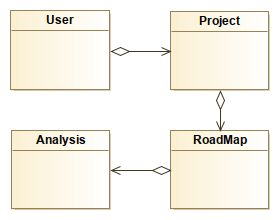
\includegraphics[scale=0.5]{img/conceptual00}
	\caption{Schema concettuale}
	\label{fig:cd-conceptual}
\end{figure}



\section{Modellazione della rete stradale}
Interesse di questo lavoro è lo studio del traffico nei pressi di un incrocio tra auto e tramvia.
Per supportare una visione più ampia, ed altre eventuali tipologie di analisi, sarà proposto un modello in grado di descrivere una generica rete di trasporti.

\subsection{Il grafo dei trasporti}
Si può pensare di modellare una rete stradale con un grafo in cui gli archi e i nodi rappresentino rispettivamente le carreggiate delle strade ed i punti di interesse come gli incroci.
Questi due concetti saranno rappresentati dagli elementi \textit{RelevantPoint} e \textit{LaneSegment}.
Nel suo caso più basilare tale definizione corrisponde precisamente con quella matematica di grafo orientato, ovvero:
$$G = (V, E)$$
Con $V$ insieme dei vertici ed $E \subseteq V \times V$ insieme di coppie ordinate di vertici\cite{data_structures}.
In figura \ref{fig:model00} sono mostrate le entità e i legami basilari tra esse: l'unico vincolo importante è che un segmento di strada deve avere come sorgente e destinazione un punto rilevante.

\begin{figure}[h]
	\centering
	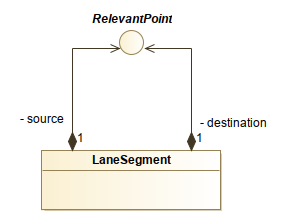
\includegraphics[scale=0.5]{img/model00}
	\caption{Entità basilari in un sistema stradale}
	\label{fig:model00}
\end{figure}

Si definisce grado di entrata in un nodo $\delta_i(v_0)$ la cardinalità del seguente insieme:
$$\{(v, v_0) \in E\}$$
Mentre il grado di uscita $\delta_o(v_0)$ è la cardinalità di:
$$\{(v_0, v) \in E\}$$

I nodi con grado di entrata o di uscita nullo hanno speciale significato in questo ambito, ovvero se dato $v_s \in V$, $\delta_i(v_s) = 0$, allora $v_s$ è un nodo di entrata nel sistema, mentre se dato $v_d \in V$, $\delta_o(v_d) = 0$, allora $v_d$ è nodo di uscita dal sistema (\ref{fig:model01}).

Siano $S$ e $D$ i rispettivi insiemi di nodi sorgente e destinazione, è stata introdotta la seguente limitazione per semplificare il lavoro di analisi:
$$v_s \in S \Rightarrow \delta_o(v_s) = 1$$
Ovvero un nodo sorgente può essere collegato ad una sola strada.\\
Questo non limita l'espressività del sistema in quanto è sufficiente dividere un nodo sorgente per ottenere la rappresentazione desiderata (\ref{fig:graph00}).
\begin{figure}[h]
	\centering
	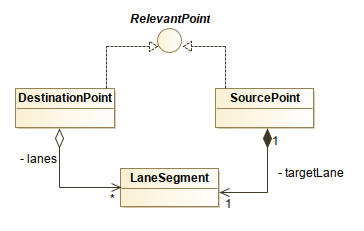
\includegraphics[scale=0.5]{img/model01}
	\caption{Sorgenti e destinazioni}
	\label{fig:model01}
\end{figure}

\begin{figure}[h]
	\centering
	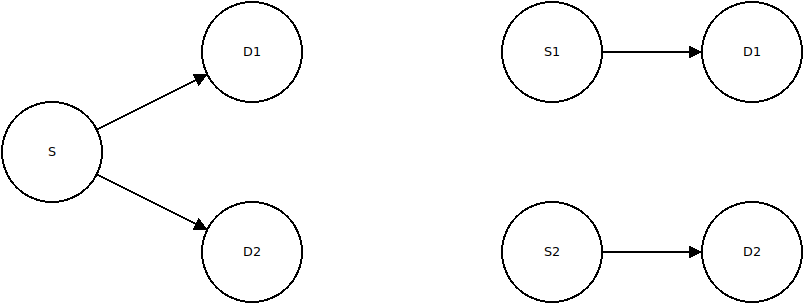
\includegraphics[scale=0.5]{img/graph00}
	\caption{Divisione di un nodo sorgente}
	\label{fig:graph00}
\end{figure}

I nodi interni alla rete invece sono realizzati da istanze della classe \textit{CrossingPoint}, che fornisce il supporto di base alla modellazione di un incrocio generico, definendo una mappa che associa ad ogni linea in entrata una o più linee in uscita: in questo modo sono coperti numerosi casi reali anche particolari, tra cui:
\begin{itemize}
	\item Impossibilità di accedere ad una strada a partire da una certa corsia.
	\item Impossibilità di effettuare inversioni ad U.
	\item Impostare alcune tratte come più o meno trafficate.
\end{itemize}

Oltre alla versione base di \textit{CrossingPoint}, che rappresenta un incrocio non arbitrato, è stata definita una versione \textit{TrafficLightCrossingPoint} che invece introduce il concetto di semaforo (\textit{TrafficLight}).
Diventa possibile associare ad ogni linea in ingresso all'incrocio un semaforo che la gestisce, in particolare sono state implementate le varianti temporizzate e a sensore: quest'ultimo caso è utile quando per esempio una linea automobilistica è interrotta da una linea tramviaria.
Vedi figura \ref{fig:model02}.

\begin{figure}[h]
	\centering
	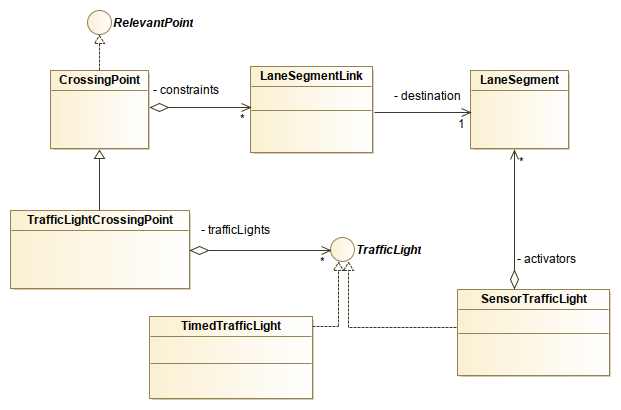
\includegraphics[scale=0.5]{img/model02}
	\caption{Modellazione di un incrocio}
	\label{fig:model02}
\end{figure}

\subsection{Configurazione}

Per gli scopi a cui è destinato, il modello mostrato non prevede particolari funzionalità operative: il suo scopo è principalmente quello di \textit{descrivere} una rete stradale.
Per poter facilmente estendere il software (per esempio con un modulo user friendly per la creazione della rete o nuove analisi non ancora previste), le entità precedentemente descritte hanno la possibilità di essere configurate con una serie arbitraria di proprietà tipizzate chiave-valore (\textit{Property}).
Sarà possibile da parte dell'utente creare una serie di proprietà e configurazioni predefinite da applicare poi ad una eventuale rete. Vedi figura \ref{fig:model03}.
Lo scopo di questo livello intermedio è quello di scaricare l'utente dalla necessità di conoscere tutte le possibili proprietà di configurazione.

\begin{figure}[h]
	\centering
	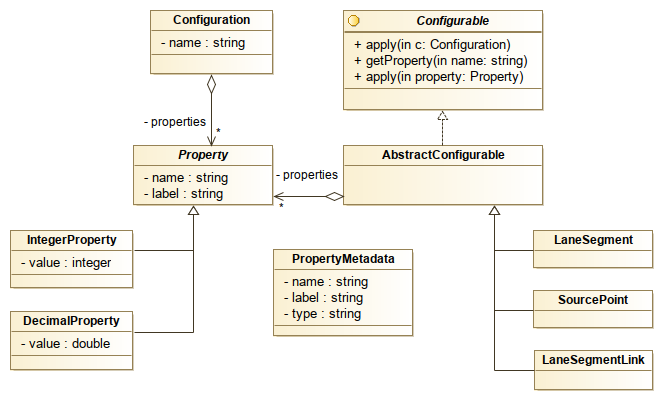
\includegraphics[scale=0.5]{img/model03}
	\caption{Configurazione}
	\label{fig:model03}
\end{figure}

La classe aggiuntiva \textit{PropertyMetadata} potrà essere utilizzata per fissare i nomi di alcune proprietà notevoli in modo da evitare errori nel tipo o nel nome al momento della definizione.



\section{Schermate dell'applicazione}
Di seguito saranno riportate alcune schermate di esempio.

\begin{figure}[h]
	\centering
	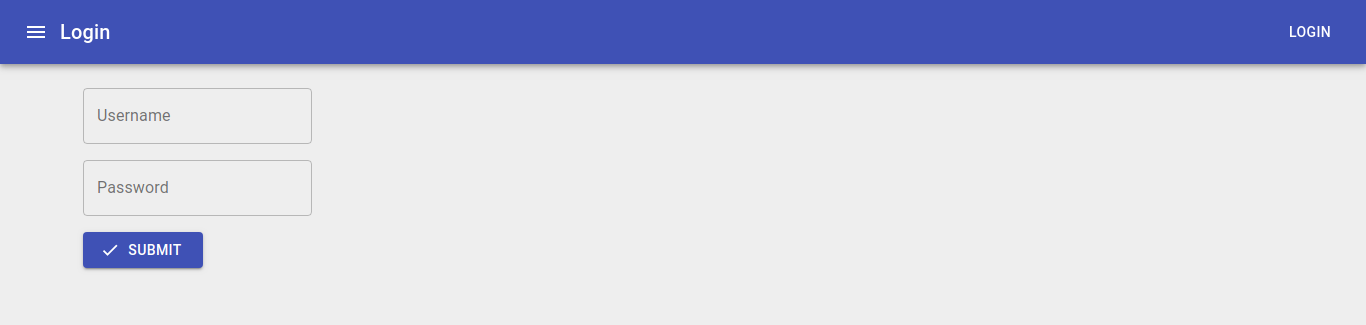
\includegraphics[width=\textwidth]{img/screen00}
	\caption{Form di login}
	\label{fig:screen00}
\end{figure}

\begin{figure}[h]
	\centering
	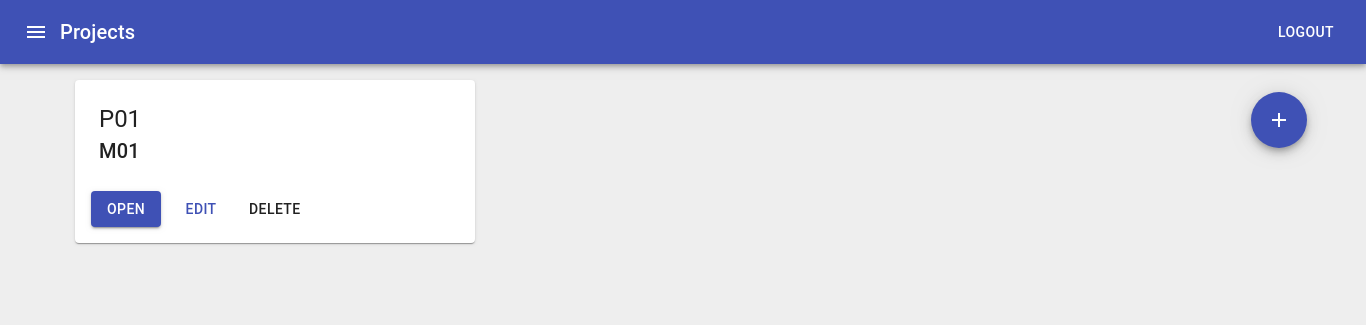
\includegraphics[width=\textwidth]{img/screen01}
	\caption{Elenco dei progetti}
	\label{fig:screen01}
\end{figure}

\begin{figure}[h]
	\centering
	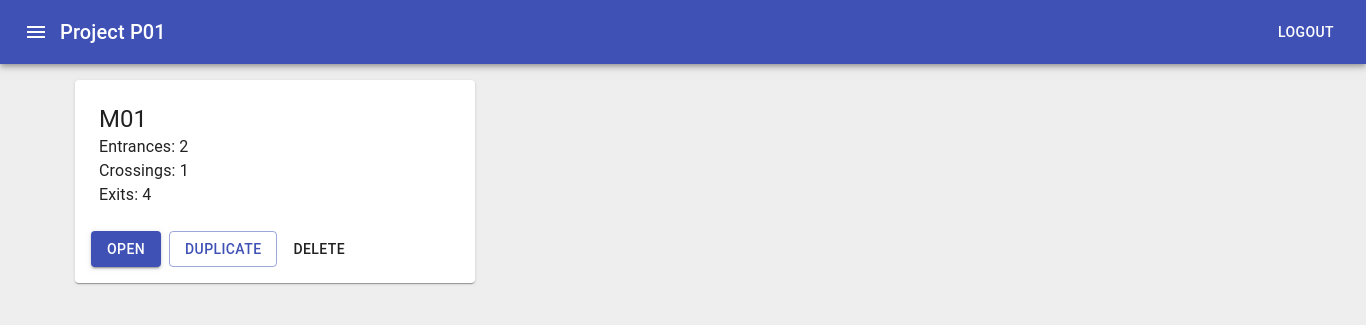
\includegraphics[width=\textwidth]{img/screen02}
	\caption{Contenuto di un progetto}
	\label{fig:screen02}
\end{figure}

\begin{figure}[h]
	\centering
	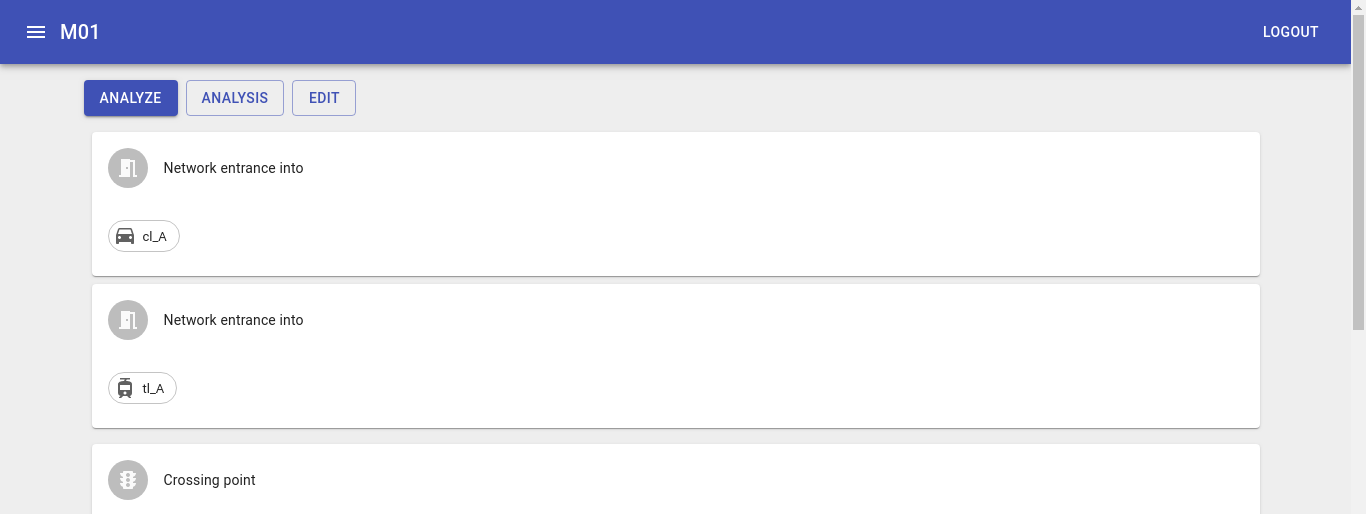
\includegraphics[width=\textwidth]{img/screen03}
	\caption{Visualizzazione di una mappa}
	\label{fig:screen03}
\end{figure}


\begin{figure}[h]
	\centering
	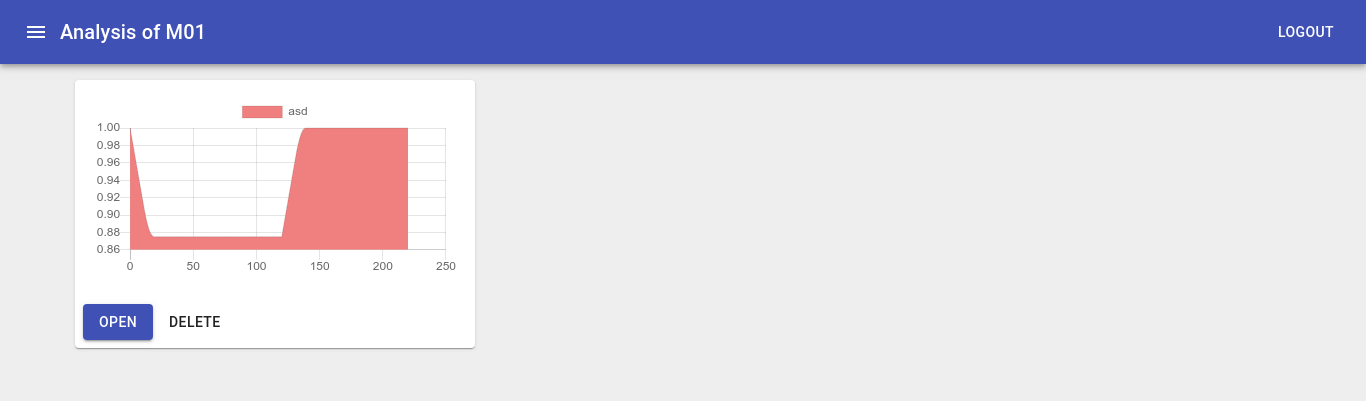
\includegraphics[width=\textwidth]{img/screen04}
	\caption{Analisi effettuate}
	\label{fig:screen04}
\end{figure}

